\documentclass[10pt]{article}
\usepackage{tikz}
\usetikzlibrary{shapes.misc}
\usepackage[margin=0cm]{geometry}
\pagestyle{empty}
\tikzstyle{every node}=[cross out, draw, red]

\begin{document}

\vspace*{\fill}
\begin{center}
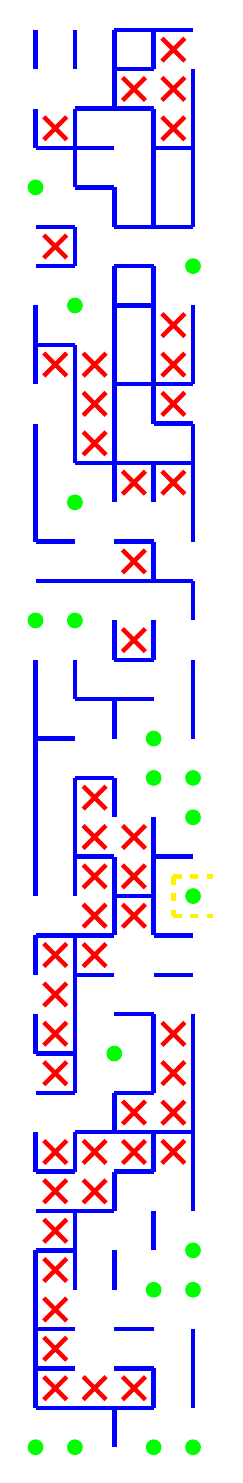
\begin{tikzpicture}[x=0.5cm, y=-0.5cm, ultra thick, blue]
% Walls
    \draw (2,0) -- (4,0);
    \draw (2,1) -- (3,1);
    \draw (1,2) -- (3,2);
    \draw (0,3) -- (2,3);
    \draw (3,3) -- (4,3);
    \draw (1,4) -- (2,4);
    \draw (0,5) -- (1,5);
    \draw (2,5) -- (4,5);
    \draw (0,6) -- (1,6);
    \draw (2,6) -- (3,6);
    \draw (2,7) -- (3,7);
    \draw (0,8) -- (1,8);
    \draw (2,9) -- (4,9);
    \draw (3,10) -- (4,10);
    \draw (1,11) -- (4,11);
    \draw (0,13) -- (1,13);
    \draw (2,13) -- (3,13);
    \draw (0,14) -- (4,14);
    \draw (2,16) -- (3,16);
    \draw (1,17) -- (3,17);
    \draw (0,18) -- (1,18);
    \draw (1,19) -- (2,19);
    \draw (1,21) -- (2,21);
    \draw (3,21) -- (4,21);
    \draw (2,22) -- (3,22);
    \draw (0,23) -- (2,23);
    \draw (3,23) -- (4,23);
    \draw (1,24) -- (2,24);
    \draw (3,24) -- (4,24);
    \draw (2,25) -- (3,25);
    \draw (0,26) -- (1,26);
    \draw (0,27) -- (1,27);
    \draw (2,27) -- (3,27);
    \draw (1,28) -- (4,28);
    \draw (0,29) -- (1,29);
    \draw (2,29) -- (3,29);
    \draw (0,30) -- (2,30);
    \draw (0,31) -- (1,31);
    \draw (0,33) -- (1,33);
    \draw (2,33) -- (3,33);
    \draw (0,34) -- (1,34);
    \draw (2,34) -- (3,34);
    \draw (0,35) -- (3,35);
    \draw (0,0) -- (0,1);
    \draw (0,2) -- (0,3);
    \draw (0,7) -- (0,9);
    \draw (0,10) -- (0,13);
    \draw (0,16) -- (0,22);
    \draw (0,23) -- (0,24);
    \draw (0,25) -- (0,26);
    \draw (0,28) -- (0,29);
    \draw (0,31) -- (0,35);
    \draw (1,0) -- (1,1);
    \draw (1,2) -- (1,4);
    \draw (1,5) -- (1,6);
    \draw (1,8) -- (1,11);
    \draw (1,16) -- (1,17);
    \draw (1,19) -- (1,22);
    \draw (1,23) -- (1,27);
    \draw (1,28) -- (1,29);
    \draw (1,30) -- (1,32);
    \draw (2,0) -- (2,2);
    \draw (2,4) -- (2,5);
    \draw (2,6) -- (2,12);
    \draw (2,15) -- (2,16);
    \draw (2,17) -- (2,18);
    \draw (2,19) -- (2,20);
    \draw (2,21) -- (2,23);
    \draw (2,27) -- (2,28);
    \draw (2,29) -- (2,30);
    \draw (2,31) -- (2,32);
    \draw (2,35) -- (2,36);
    \draw (3,0) -- (3,1);
    \draw (3,2) -- (3,5);
    \draw (3,6) -- (3,10);
    \draw (3,11) -- (3,12);
    \draw (3,13) -- (3,14);
    \draw (3,15) -- (3,16);
    \draw (3,20) -- (3,23);
    \draw (3,25) -- (3,27);
    \draw (3,28) -- (3,29);
    \draw (3,30) -- (3,31);
    \draw (3,34) -- (3,35);
    \draw (4,1) -- (4,5);
    \draw (4,7) -- (4,9);
    \draw (4,10) -- (4,13);
    \draw (4,14) -- (4,15);
    \draw (4,16) -- (4,18);
    \draw (4,25) -- (4,30);
    \draw (4,33) -- (4,35);
% Pillars
    \fill[green] (0,4) circle(0.2);
    \fill[green] (4,6) circle(0.2);
    \fill[green] (1,7) circle(0.2);
    \fill[green] (1,12) circle(0.2);
    \fill[green] (0,15) circle(0.2);
    \fill[green] (1,15) circle(0.2);
    \fill[green] (3,18) circle(0.2);
    \fill[green] (3,19) circle(0.2);
    \fill[green] (4,19) circle(0.2);
    \fill[green] (4,20) circle(0.2);
    \fill[green] (4,22) circle(0.2);
    \fill[green] (2,26) circle(0.2);
    \fill[green] (4,31) circle(0.2);
    \fill[green] (3,32) circle(0.2);
    \fill[green] (4,32) circle(0.2);
    \fill[green] (0,36) circle(0.2);
    \fill[green] (1,36) circle(0.2);
    \fill[green] (3,36) circle(0.2);
    \fill[green] (4,36) circle(0.2);
% Inner points in accessible cul-de-sacs
    \node at (3.5,0.5) {};
    \node at (2.5,1.5) {};
    \node at (3.5,1.5) {};
    \node at (0.5,2.5) {};
    \node at (3.5,2.5) {};
    \node at (0.5,5.5) {};
    \node at (3.5,7.5) {};
    \node at (0.5,8.5) {};
    \node at (1.5,8.5) {};
    \node at (3.5,8.5) {};
    \node at (1.5,9.5) {};
    \node at (3.5,9.5) {};
    \node at (1.5,10.5) {};
    \node at (2.5,11.5) {};
    \node at (3.5,11.5) {};
    \node at (2.5,13.5) {};
    \node at (2.5,15.5) {};
    \node at (1.5,19.5) {};
    \node at (1.5,20.5) {};
    \node at (2.5,20.5) {};
    \node at (1.5,21.5) {};
    \node at (2.5,21.5) {};
    \node at (1.5,22.5) {};
    \node at (2.5,22.5) {};
    \node at (0.5,23.5) {};
    \node at (1.5,23.5) {};
    \node at (0.5,24.5) {};
    \node at (0.5,25.5) {};
    \node at (3.5,25.5) {};
    \node at (0.5,26.5) {};
    \node at (3.5,26.5) {};
    \node at (2.5,27.5) {};
    \node at (3.5,27.5) {};
    \node at (0.5,28.5) {};
    \node at (1.5,28.5) {};
    \node at (2.5,28.5) {};
    \node at (3.5,28.5) {};
    \node at (0.5,29.5) {};
    \node at (1.5,29.5) {};
    \node at (0.5,30.5) {};
    \node at (0.5,31.5) {};
    \node at (0.5,32.5) {};
    \node at (0.5,33.5) {};
    \node at (0.5,34.5) {};
    \node at (1.5,34.5) {};
    \node at (2.5,34.5) {};
% Entry-exit paths without intersections
    \draw[dashed, yellow] (3.5,21.5) -- (4.5,21.5);
    \draw[dashed, yellow] (3.5,22.5) -- (4.5,22.5);
    \draw[dashed, yellow] (3.5,21.5) -- (3.5,22.5);
\end{tikzpicture}
\end{center}
\vspace*{\fill}

\end{document}
